\smallframetitle

\section{Semaine du 21/05/24 au 27/05/24}
\insertsectionframe

\subsection{Statistiques stations de bases - départements}
\insertsubsectionframe

\begin{frame}{Méthodologie}
    On va utiliser une base de donnée complémentaire, reprise de celle trouvée l'année dernière.

    \begin{block}{Une nouvelle base de donnée\footnotemark[1]}
        Cette base de donnée renseigne, par département, la \textbf{superficie} (en $\unit{km^2}$), la \textbf{population} et la \textbf{densité de population} au $\unit{km^2}$.
    \end{block}
    
    A partir de cette base, on va donc pouvoir extraire le nombre d'habitants par stations (normalisé par la taille du département) et la densité de station par département.

    \begin{block}{Calcul du nombre d'habitants par stations normalisé}
        Soit $\lambda$ le nombre d'habitants par stations, par $\unit{km^2}$. Tout d'abord, on se donne $\gamma$, le rapport entre le nombre d'habitant et la surface du département, qui est donné par la densité de population.
        Ensuite, on calcule notre résultat comme suit :$$\lambda = \gamma\times\frac{1}{\text{nombre de stations du département}}$$
    \end{block}

    \footnotetext[1]{\url{https://france.ousuisje.com/departements/classement/superficie.php}}
\end{frame}

\begin{frame}{Nombre d'habitants par stations non normalisé}
    C'est le même calcul que précédemment, sauf qu'à la place de $\gamma$, on utilise simplement la population du département.
    \begin{figure}
        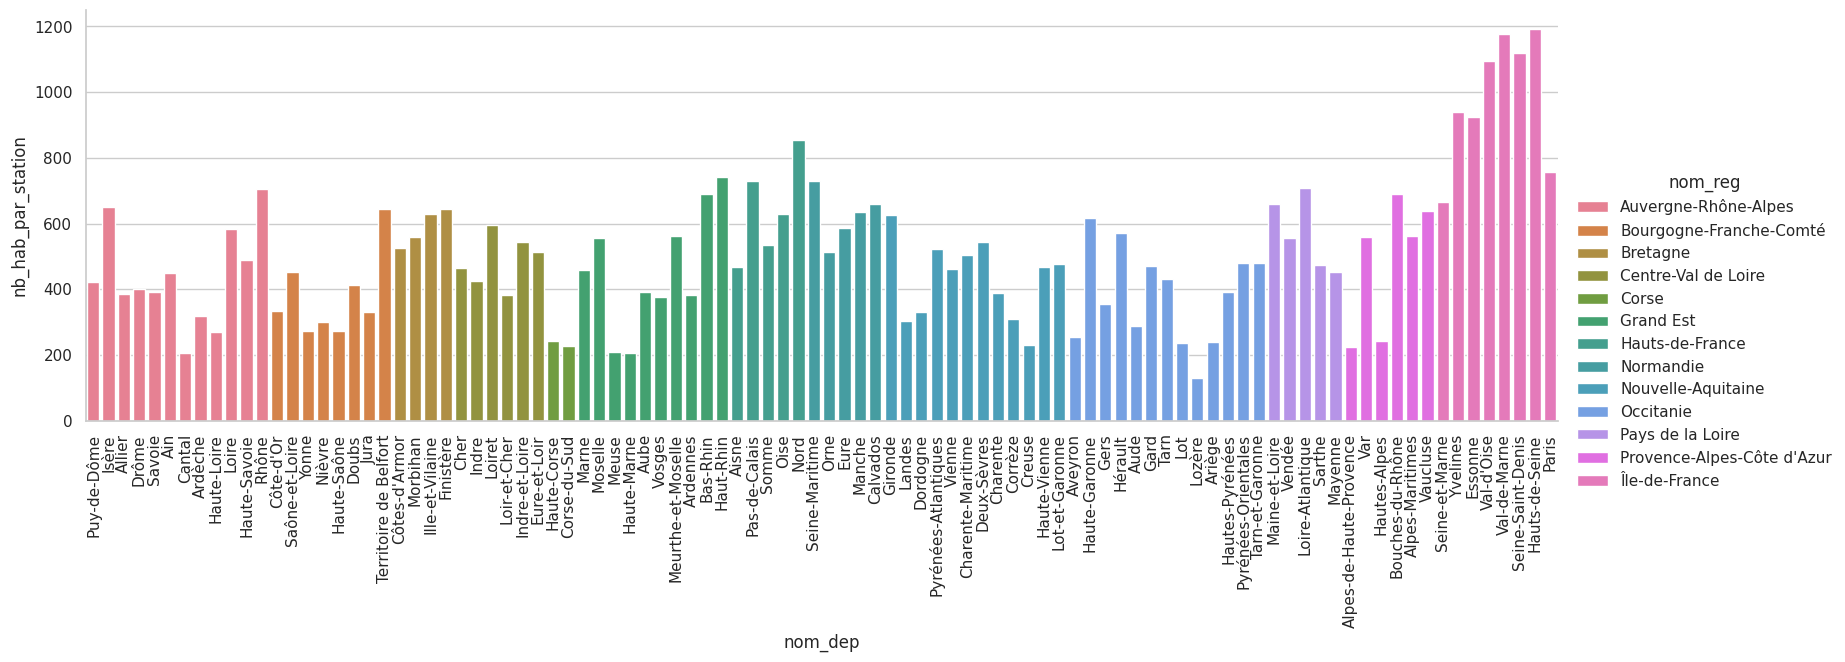
\includegraphics[width=0.9\paperwidth]{images/barplots/nb_hab_par_station_par_dep.png}
        \caption{\label{fig:nb_hap_par_stat_par_dep}Répartition du nombre d'habitants par station, en fonction du département}
    \end{figure}
\end{frame}

\begin{frame}{Nombre d'habitants par stations normalisé (1/2)}
    \begin{figure}
        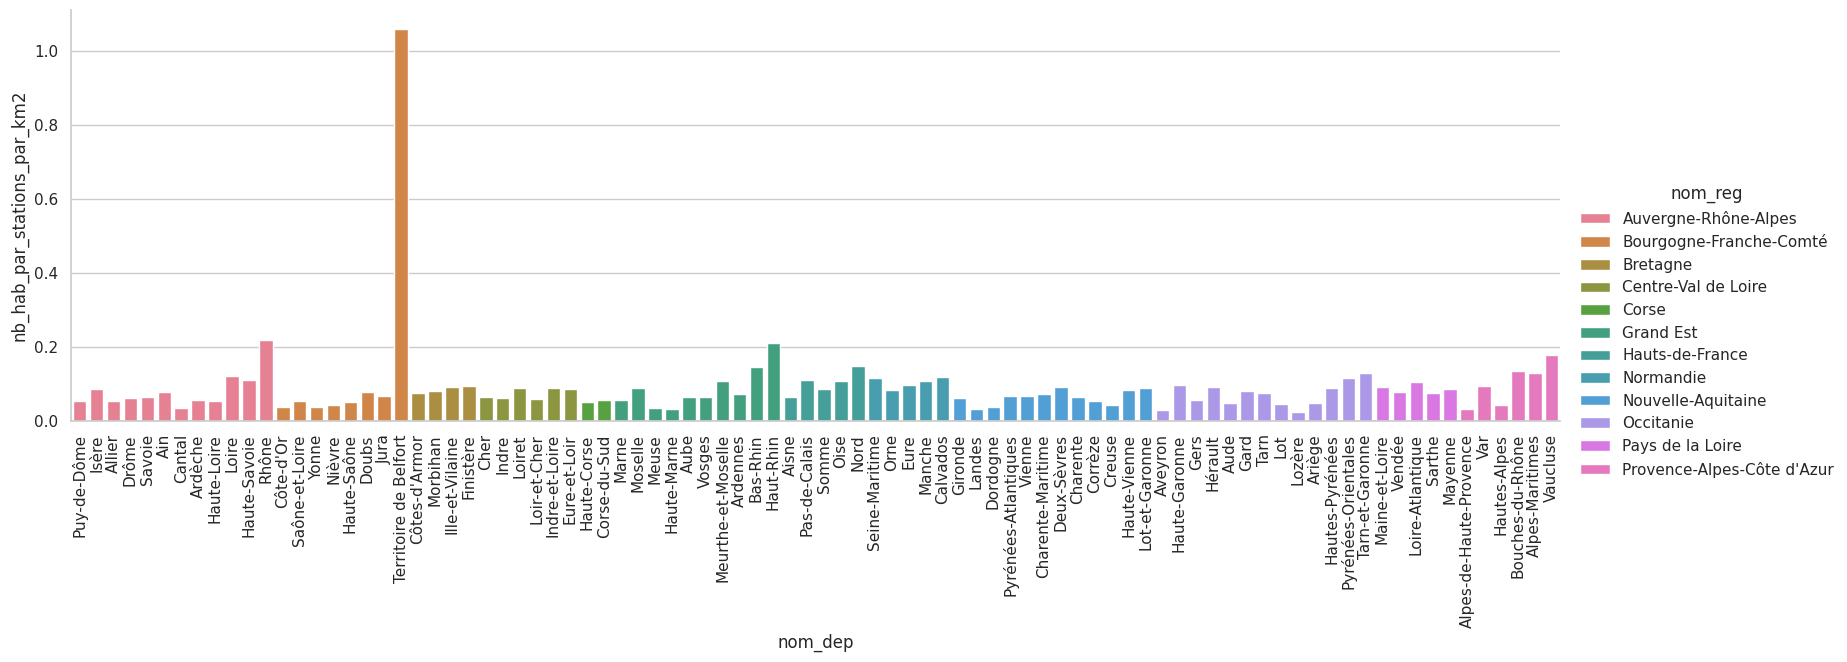
\includegraphics[width=0.9\paperwidth]{images/barplots/nb_hab_par_stations_par_km2_sansIDF.png}
        \caption{\label{fig:nb_hap_par_stat_par_dep_norm_ssIDF}Répartition du nombre d'habitants par station, en fonction du département (normalisé), sans l'Île-de-France}
    \end{figure}
\end{frame}

\begin{frame}{Nombre d'habitants par stations normalisé (2/2)}
    \begin{figure}
        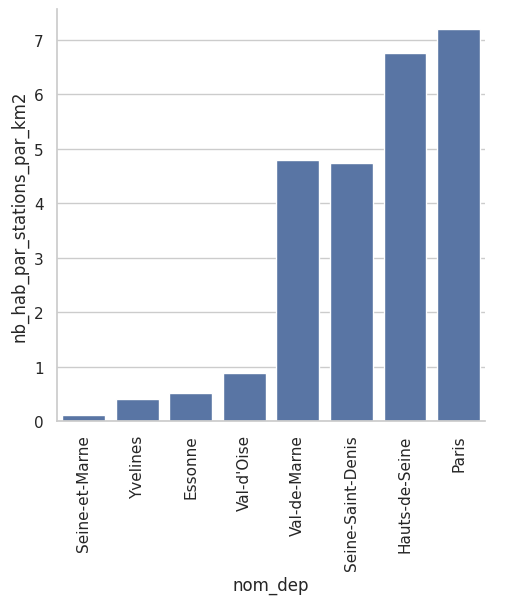
\includegraphics[height=0.55\paperheight]{images/barplots/nb_hab_par_stations_par_km2_IDF.png}
        \caption{\label{fig:nb_hap_par_stat_par_dep_norm_IDF}Répartition du nombre d'habitants par station, en fonction du département (normalisé), sur l'Île-de-France}
    \end{figure}
\end{frame}

\begin{frame}{Densité de stations (1/2)}
    \begin{figure}
        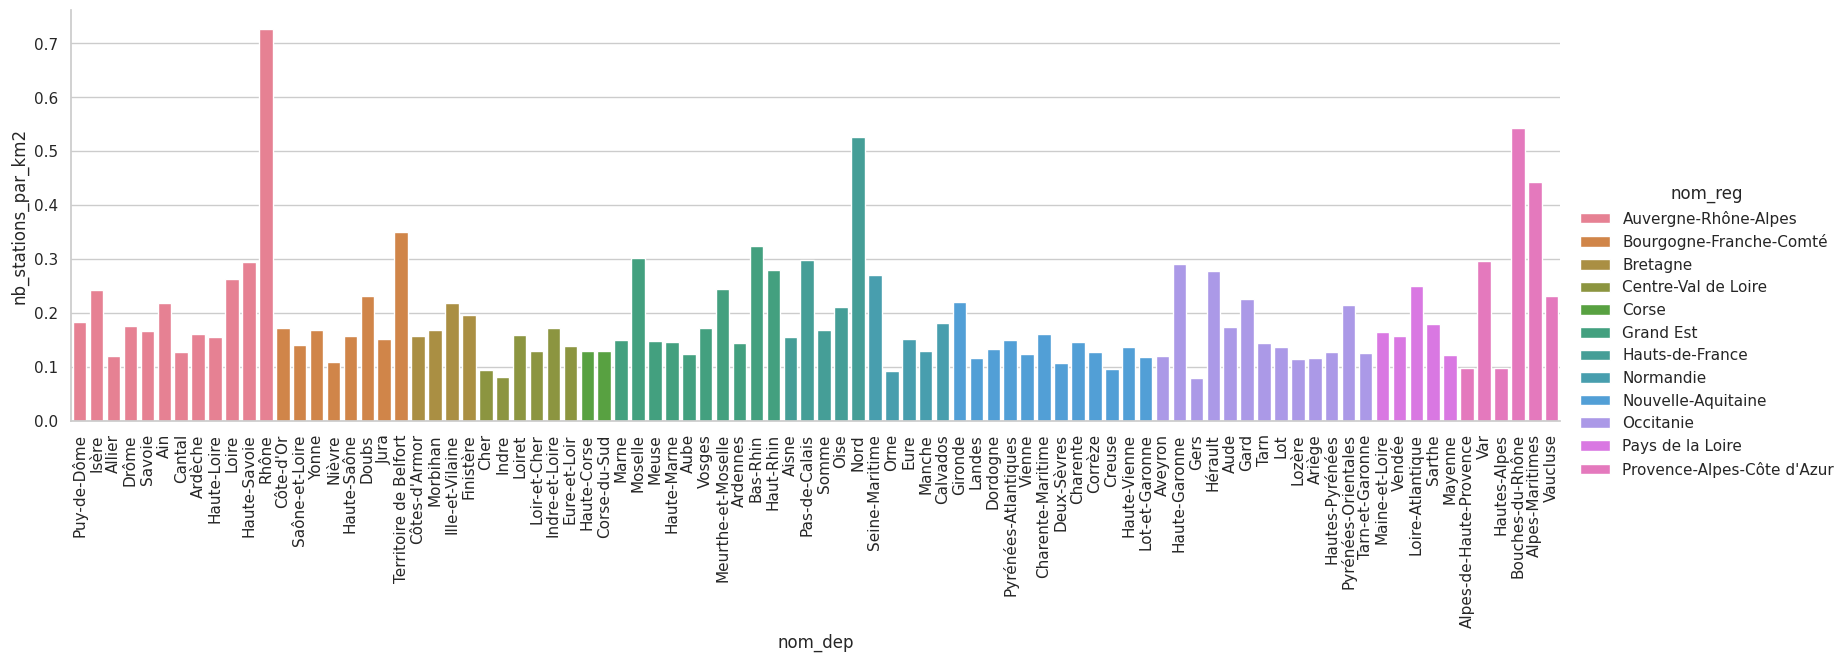
\includegraphics[width=0.9\paperwidth]{images/barplots/densite_station_par_dep_sansIDF.png}
        \caption{\label{fig:densite_stat_ssIDF}Nombre de stations de base au $\unit{km^2}$, sans l'Île-de-France}
    \end{figure}
\end{frame}

\begin{frame}{Densité de stations (2/2)}
    \begin{figure}
        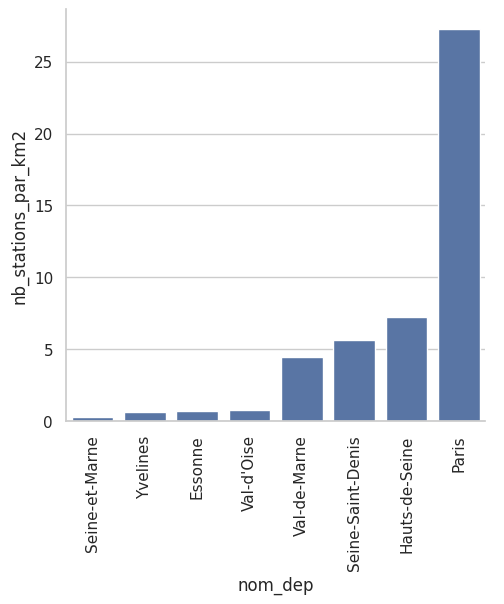
\includegraphics[height=0.55\paperheight]{images/barplots/densite_station_par_dep_IDF.png}
        \caption{\label{fig:densite_stat_IDF}Nombre de stations de base au $\unit{km^2}$, sur l'Île-de-France}
    \end{figure}
\end{frame}

\begin{frame}{Fréquences d'émission des stations 5G}
    \begin{figure}
        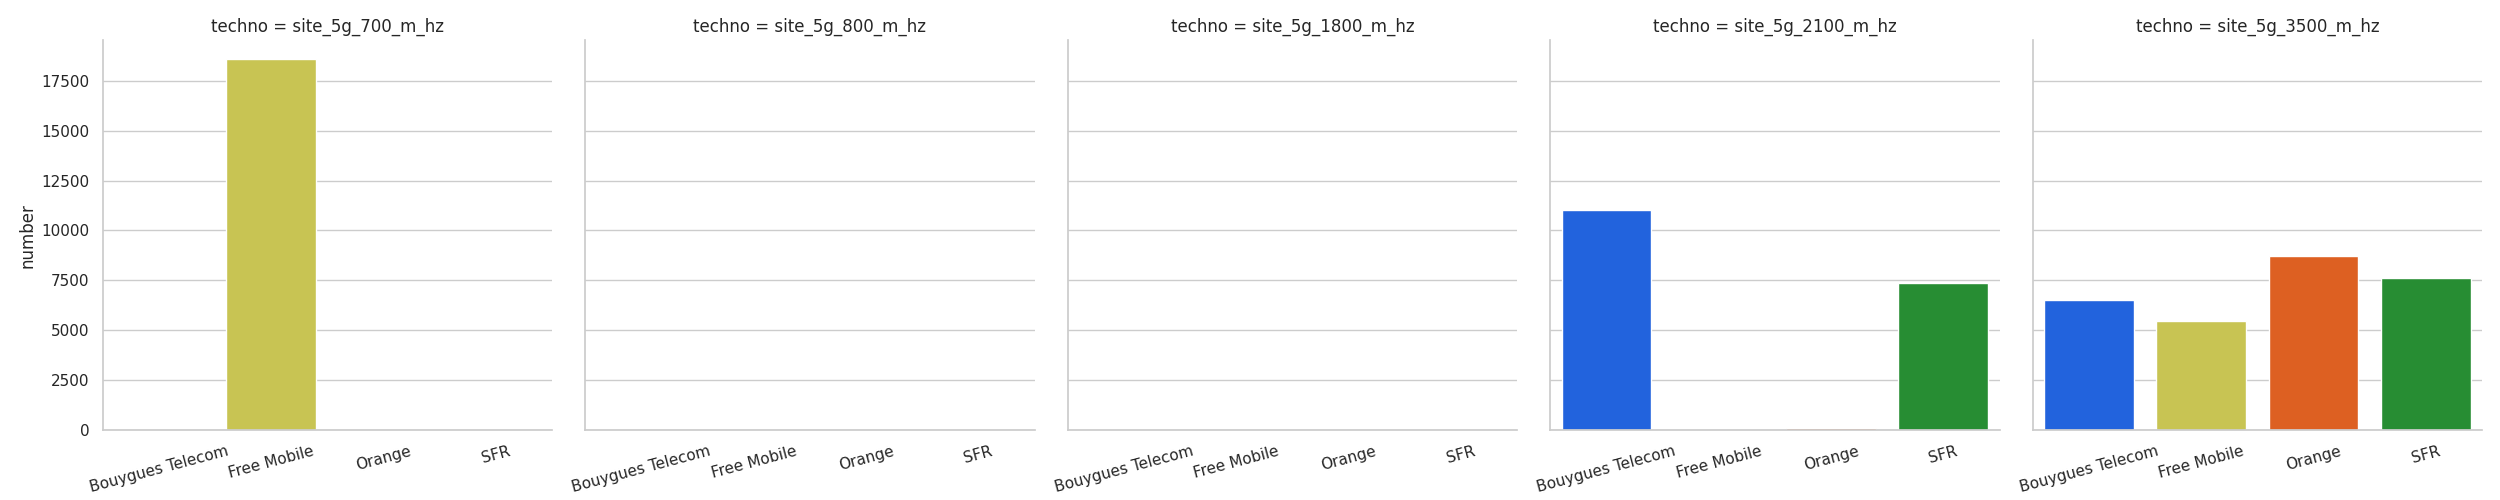
\includegraphics[width=0.9\paperwidth]{images/barplots/5G_freq.png}
        \caption{\label{fig:5g_freq}Répartition des fréquences d'émission des stations 5G, en fonction des opérateurs}
    \end{figure}
\end{frame}

\subsection{Détection de voisins - méthode PAQUIRY}
\insertsubsectionframe

\begin{frame}{Principe général}
    La recherche de voisins va s'articuler atour de deux axes :
    \begin{block}{Triangulation de Delaunay}
        On crée un graphe de voisinage grâce à la triangulation de Delaunay. Ceci nous donne donc, pour chaque station de base, une liste de voisins potentiels.
        Il faut ensuite vérifier que ce sont bien des voisins réels.
    \end{block}
    \begin{block}{Critères de sélection}
        Pour être sûr qu'un voisin est un voisin réel on applique trois critères, dans l'ordre suivant :
        \begin{enumerate}
            \item la distance maximale ;
            \item le plus proche voisin dans un cadrant ;
            \item l'angle minimum entre deux voisins.
        \end{enumerate}
    \end{block}
    Cette méthode a été élaborée par Delphine PAQUIRY l'été dernier.
\end{frame}

\begin{frame}{Critère de distance}
    \begin{columns}
        \begin{column}{0.4\paperwidth}
            \begin{block}{Principe}
                Ici, on élimine tous les voisins qui sont distants de plus de $\unit[15]{km}$.
            \end{block}
            \begin{block}{Intérêt du critère}
                Il est logique de penser que deux stations trop éloignées géographiquement ne sont pas voisines.
            \end{block}
        \end{column}
        \begin{column}{0.55\paperwidth}
            \begin{figure}
                \boxed{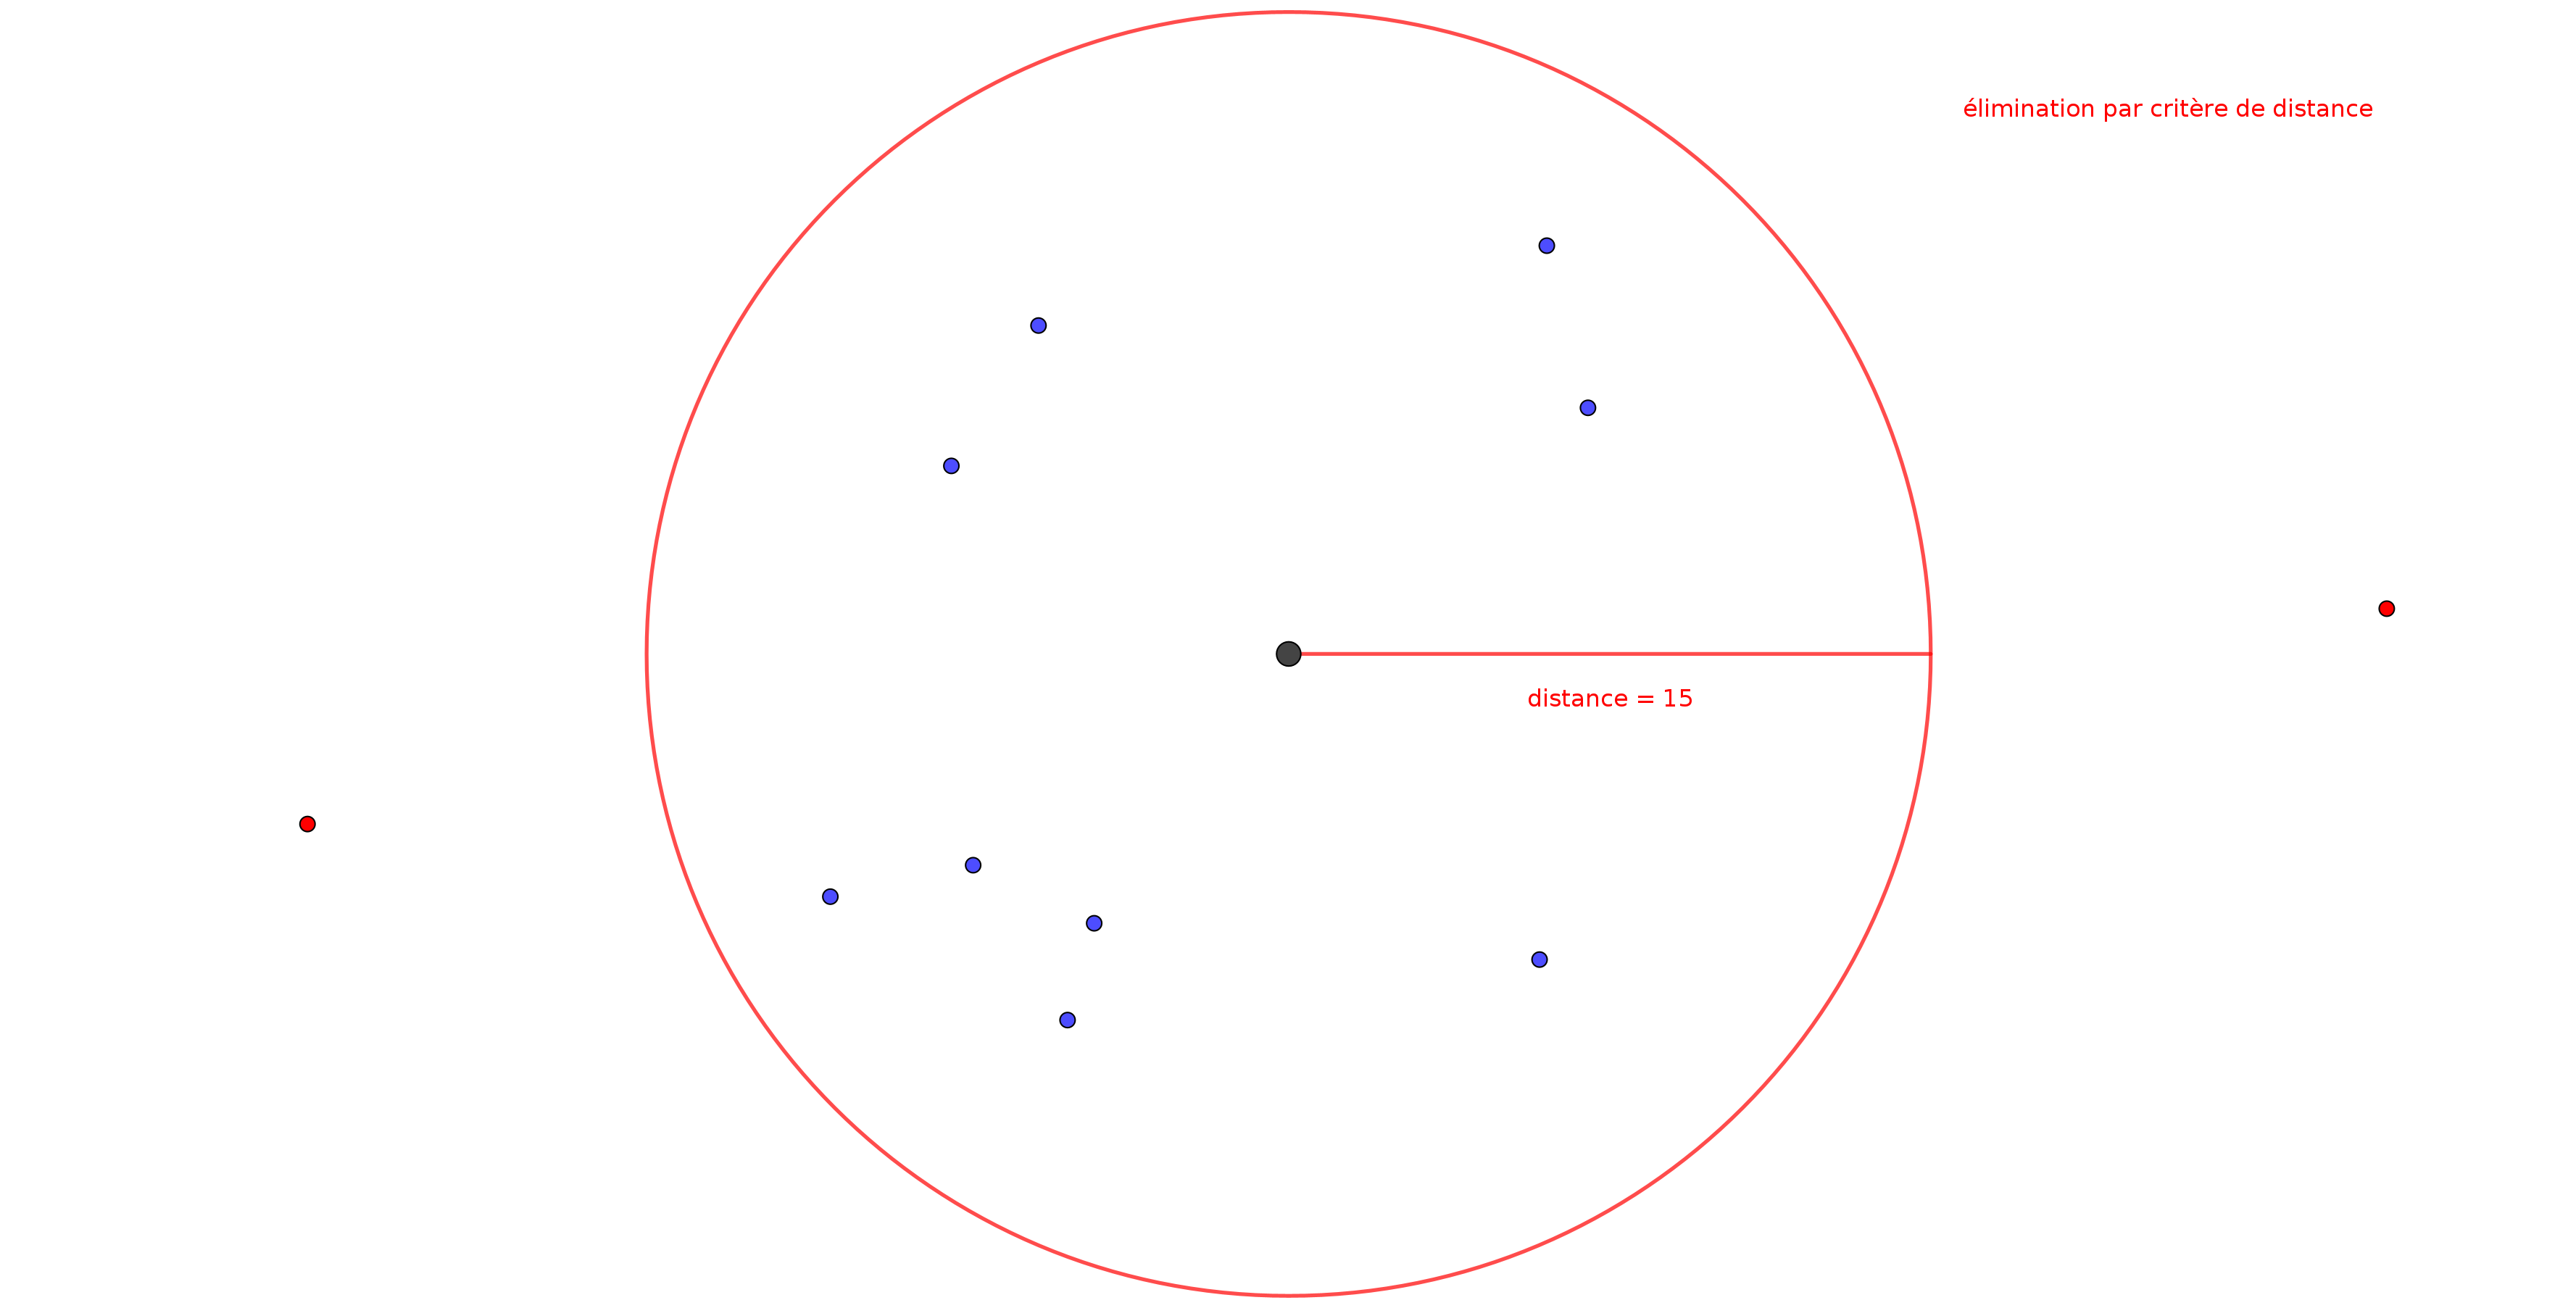
\includegraphics[width=0.5\paperwidth]{images/criteria_illustrations/distance.png}}
                \caption{\label{fig:distance_crit}Illustration du critère de distance}
            \end{figure}
        \end{column}
    \end{columns}
\end{frame}

\begin{frame}{Critère des cadrants}
    \begin{columns}
        \begin{column}{0.4\paperwidth}
            \begin{block}{Principe}
                Ici, on ne garde que le plus proche voisin dans un cadrant. On a choisi 6 cadrants car c'est le chiffre qui nous donne les meilleurs résultats.
            \end{block}
            \begin{block}{Intérêt du critère}
                On évite les effets de cluster.
            \end{block}
        \end{column}
        \begin{column}{0.55\paperwidth}
            \begin{figure}
                \boxed{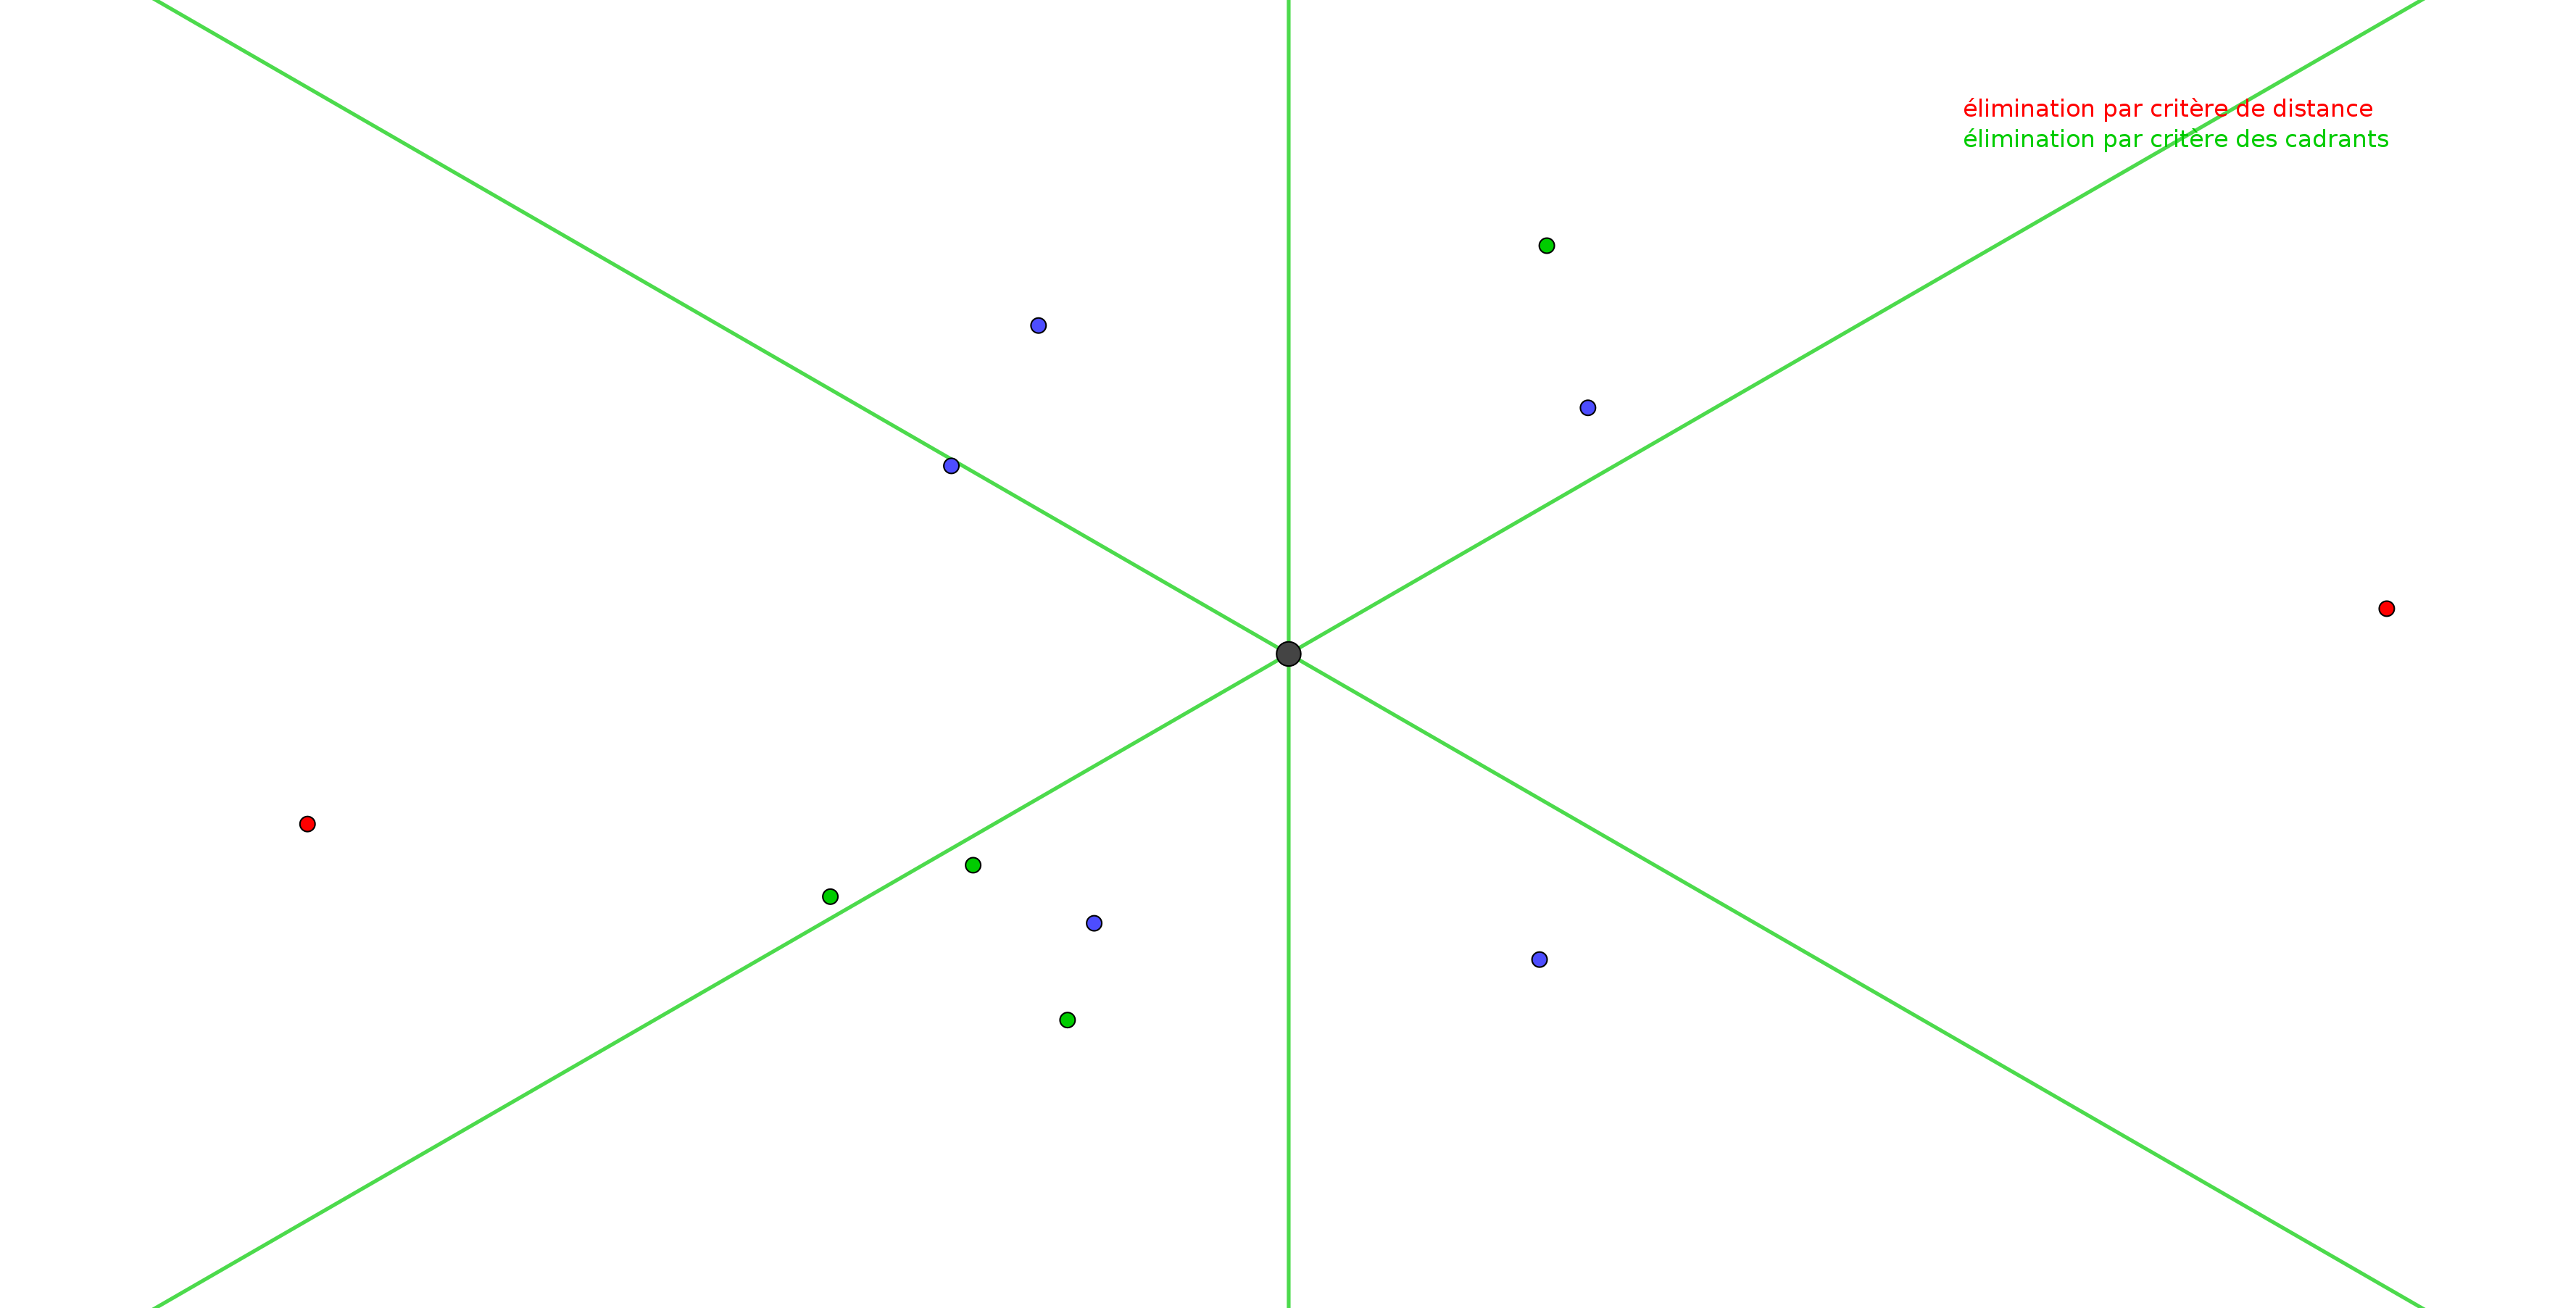
\includegraphics[width=0.5\paperwidth]{images/criteria_illustrations/cadrants.png}}
                \caption{\label{fig:cadrants_crit}Illustration du critère des cadrants}
            \end{figure}
        \end{column}
    \end{columns}
\end{frame}

\begin{frame}{Critère de l'angle}
    \begin{columns}
        \begin{column}{0.4\paperwidth}
            \begin{block}{Principe}
                Ici, si deux voisins sont séparés d'un angle inférieur à $30^{\circ}$, on ne garde que le plus proche. Cette valeur d'angle est arbitraire et pourrait être variable en fonction de l'urbanité de la station.
            \end{block}
            \begin{block}{Intérêt du critère}
                Si deux stations sont trop proches angulairement parlant, la plus proche fait écran par rapport à la plus éloignée.
            \end{block}
        \end{column}
        \begin{column}{0.55\paperwidth}
            \begin{figure}
                \boxed{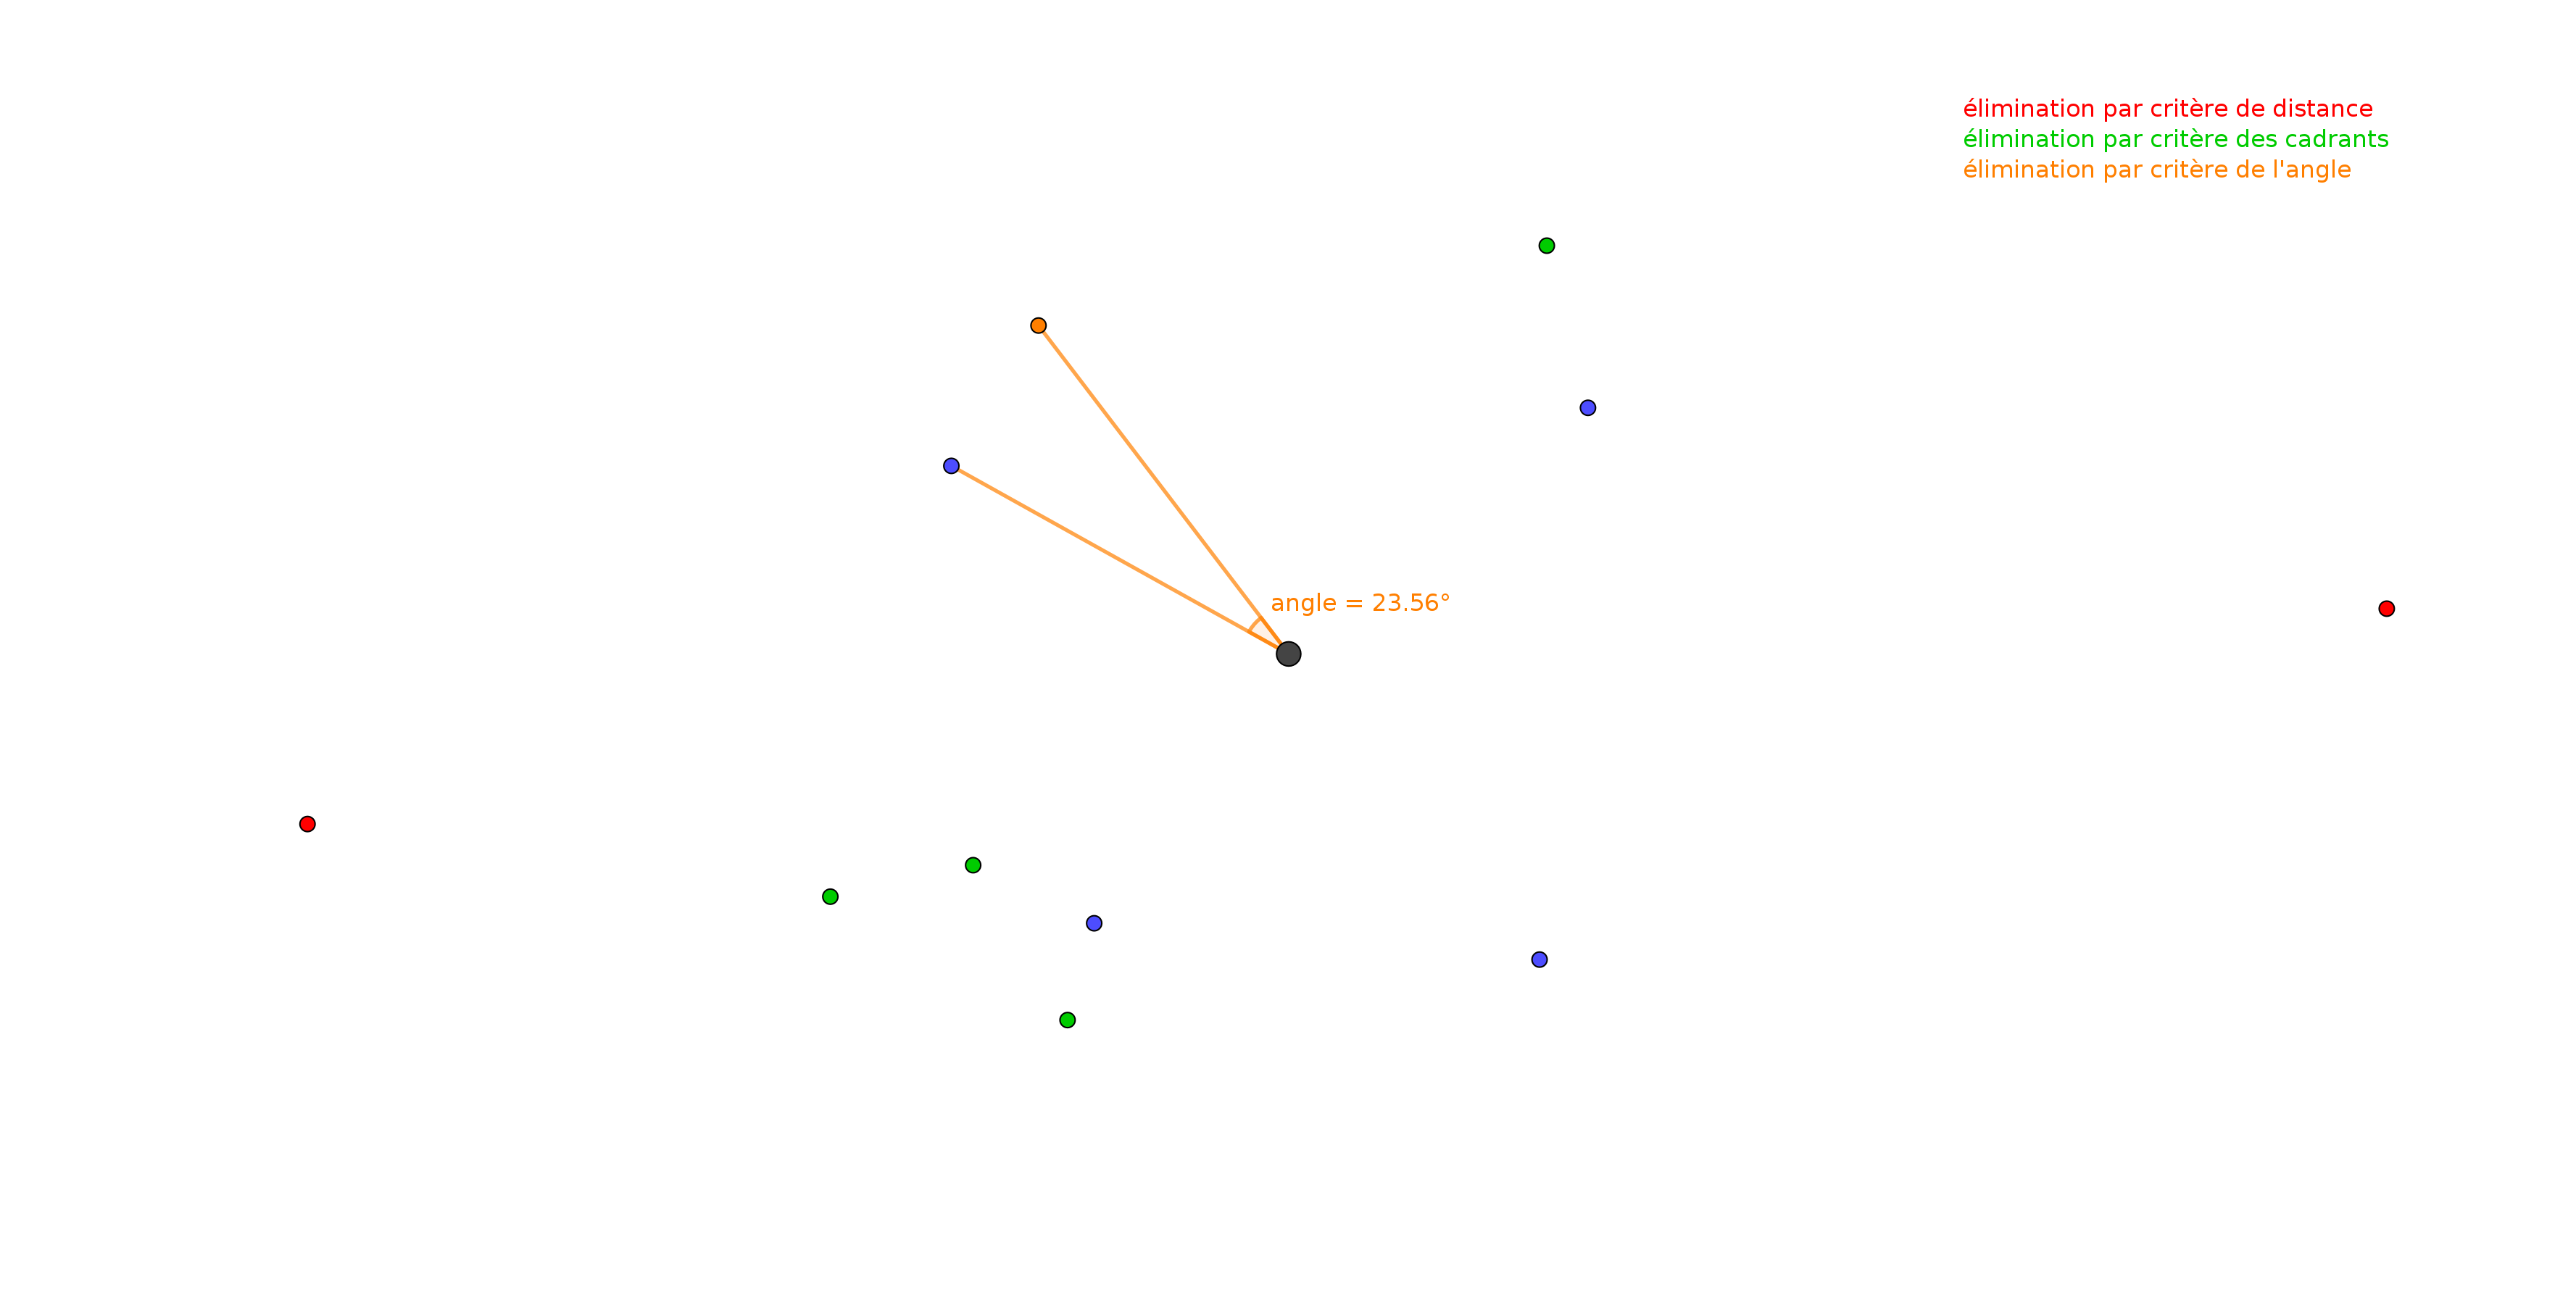
\includegraphics[width=0.5\paperwidth]{images/criteria_illustrations/angle.png}}
                \caption{\label{fig:angle_crit}Illustration du critère de l'angle}
            \end{figure}
        \end{column}
    \end{columns}
\end{frame}

\begin{frame}{Voisins réels}
    Voici donc ce que l'on obtient à la fin, un graphe de voisinage :
    \begin{figure}
        \boxed{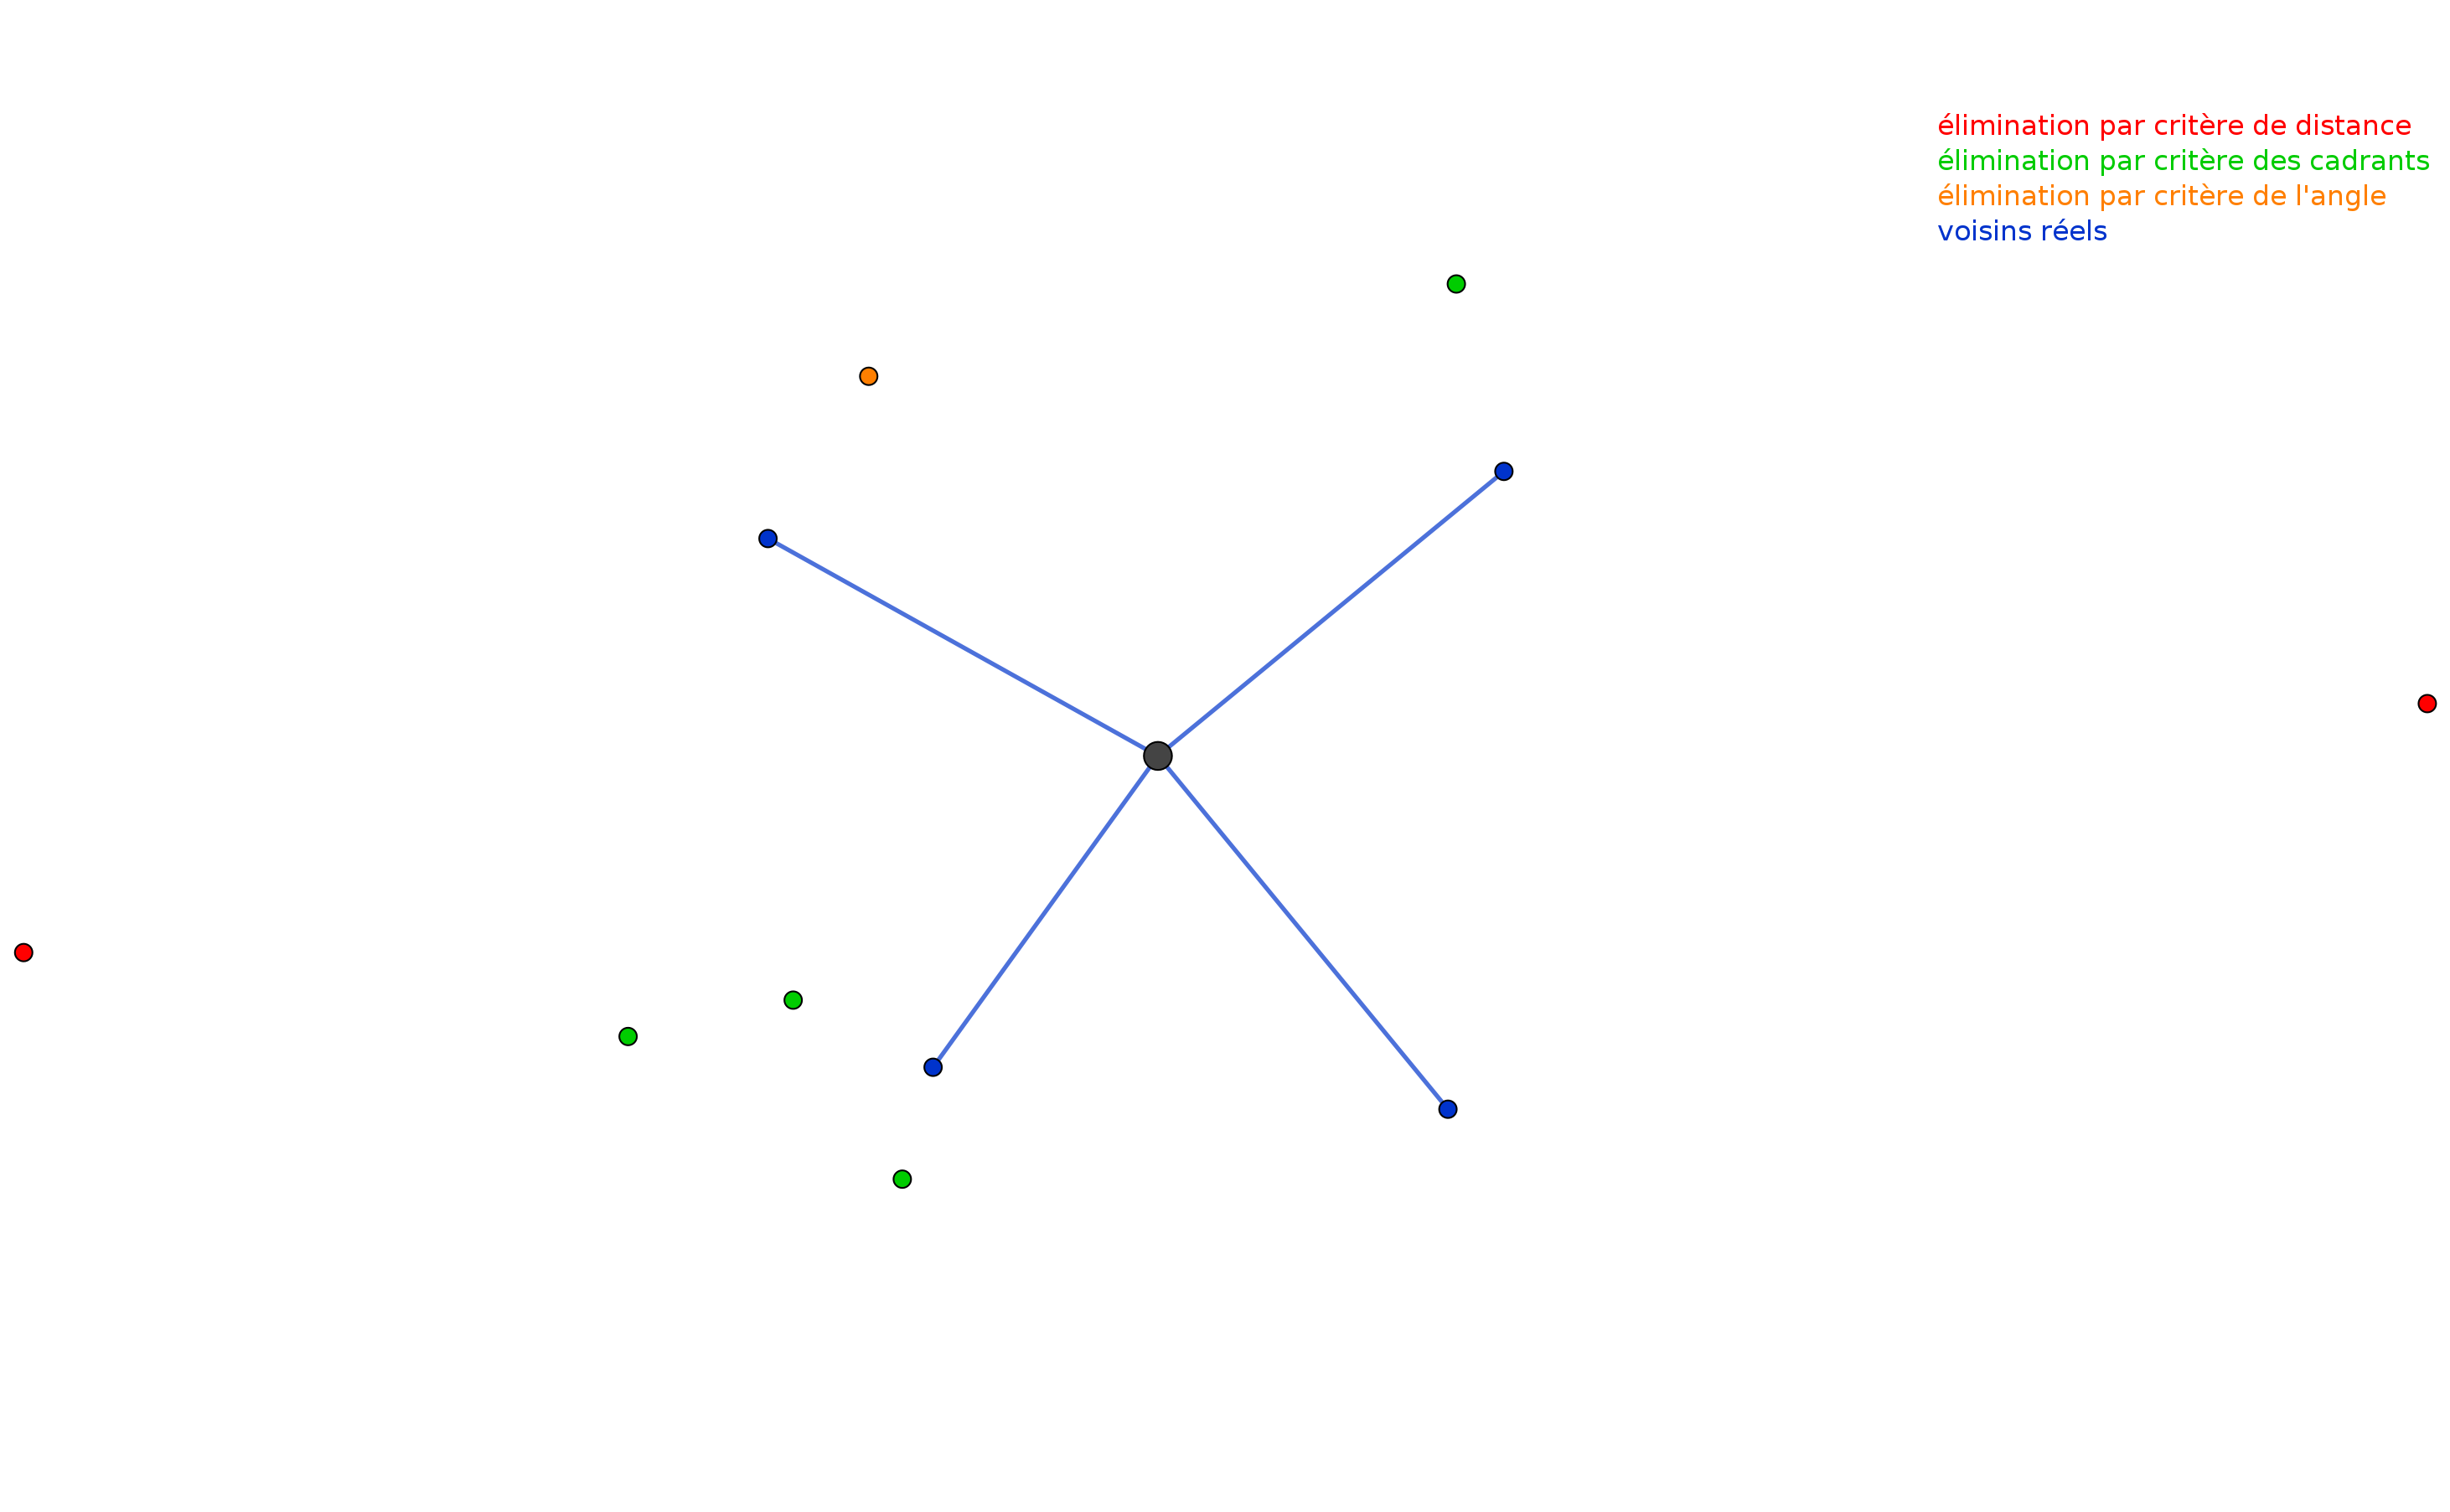
\includegraphics[height=0.55\paperheight]{images/criteria_illustrations/final.png}}
        \caption{\label{fig:result_crit}Résultat final - voisins réels}
    \end{figure}
\end{frame}

\subsection{Détection automatique des villes}
\insertsubsectionframe

\begin{frame}{DBScan}
    \begin{block}{Principe}
        \begin{itemize}
            \item Méthode de référence de la classification à densité (détection de clusters en se basant sur la concentration de points);
            \item Se base sur deux paramètres : $\varepsilon$ et $n_{min}$ qui caractérisent respectivement la distance maximale pour que deux points soient considérés \og proches \fg{} et la quantité minimale de points proches pour qu'un cluster soit créé.
        \end{itemize}
    \end{block}

    \begin{block}{Inconvénients}
        \begin{itemize}
            \item Le choix du paramètre $\varepsilon$ est hasardeux;
            \item Ne se comporte pas bien avec des jeux de données avec des clusters de densité variable (certains clusters avec des points plus rapprochés que d'autres);
            \item Réagit mal au bruit;
            \item Est binaire : un point appartient ou n'appartient pas à un cluster, pas d'entre deux.
        \end{itemize}
    \end{block}
\end{frame}

\begin{frame}{Fonctionnement DBScan (1/2)}

    \begin{columns}
        \begin{column}{0.40\textwidth}
            \begin{block}{Etape 0 : Initialisation}
                Soient n points de $\mathbb{R}^p$, $\epsilon \in \mathbb{R}$ et $n_{min} \in \mathbb{N}$.

                Ici, on prend $n_{min}=3$ et $\epsilon=2$
            \end{block}

            \begin{block}{Etape 1 - Les voisins}
                Pour chaque point, on cherche tous les points à une distance inférieure à $\epsilon$ (dont lui même). On les appelera les voisins.
            \end{block}
        \end{column}

        \begin{column}{0.60\textwidth}
            \begin{figure}
                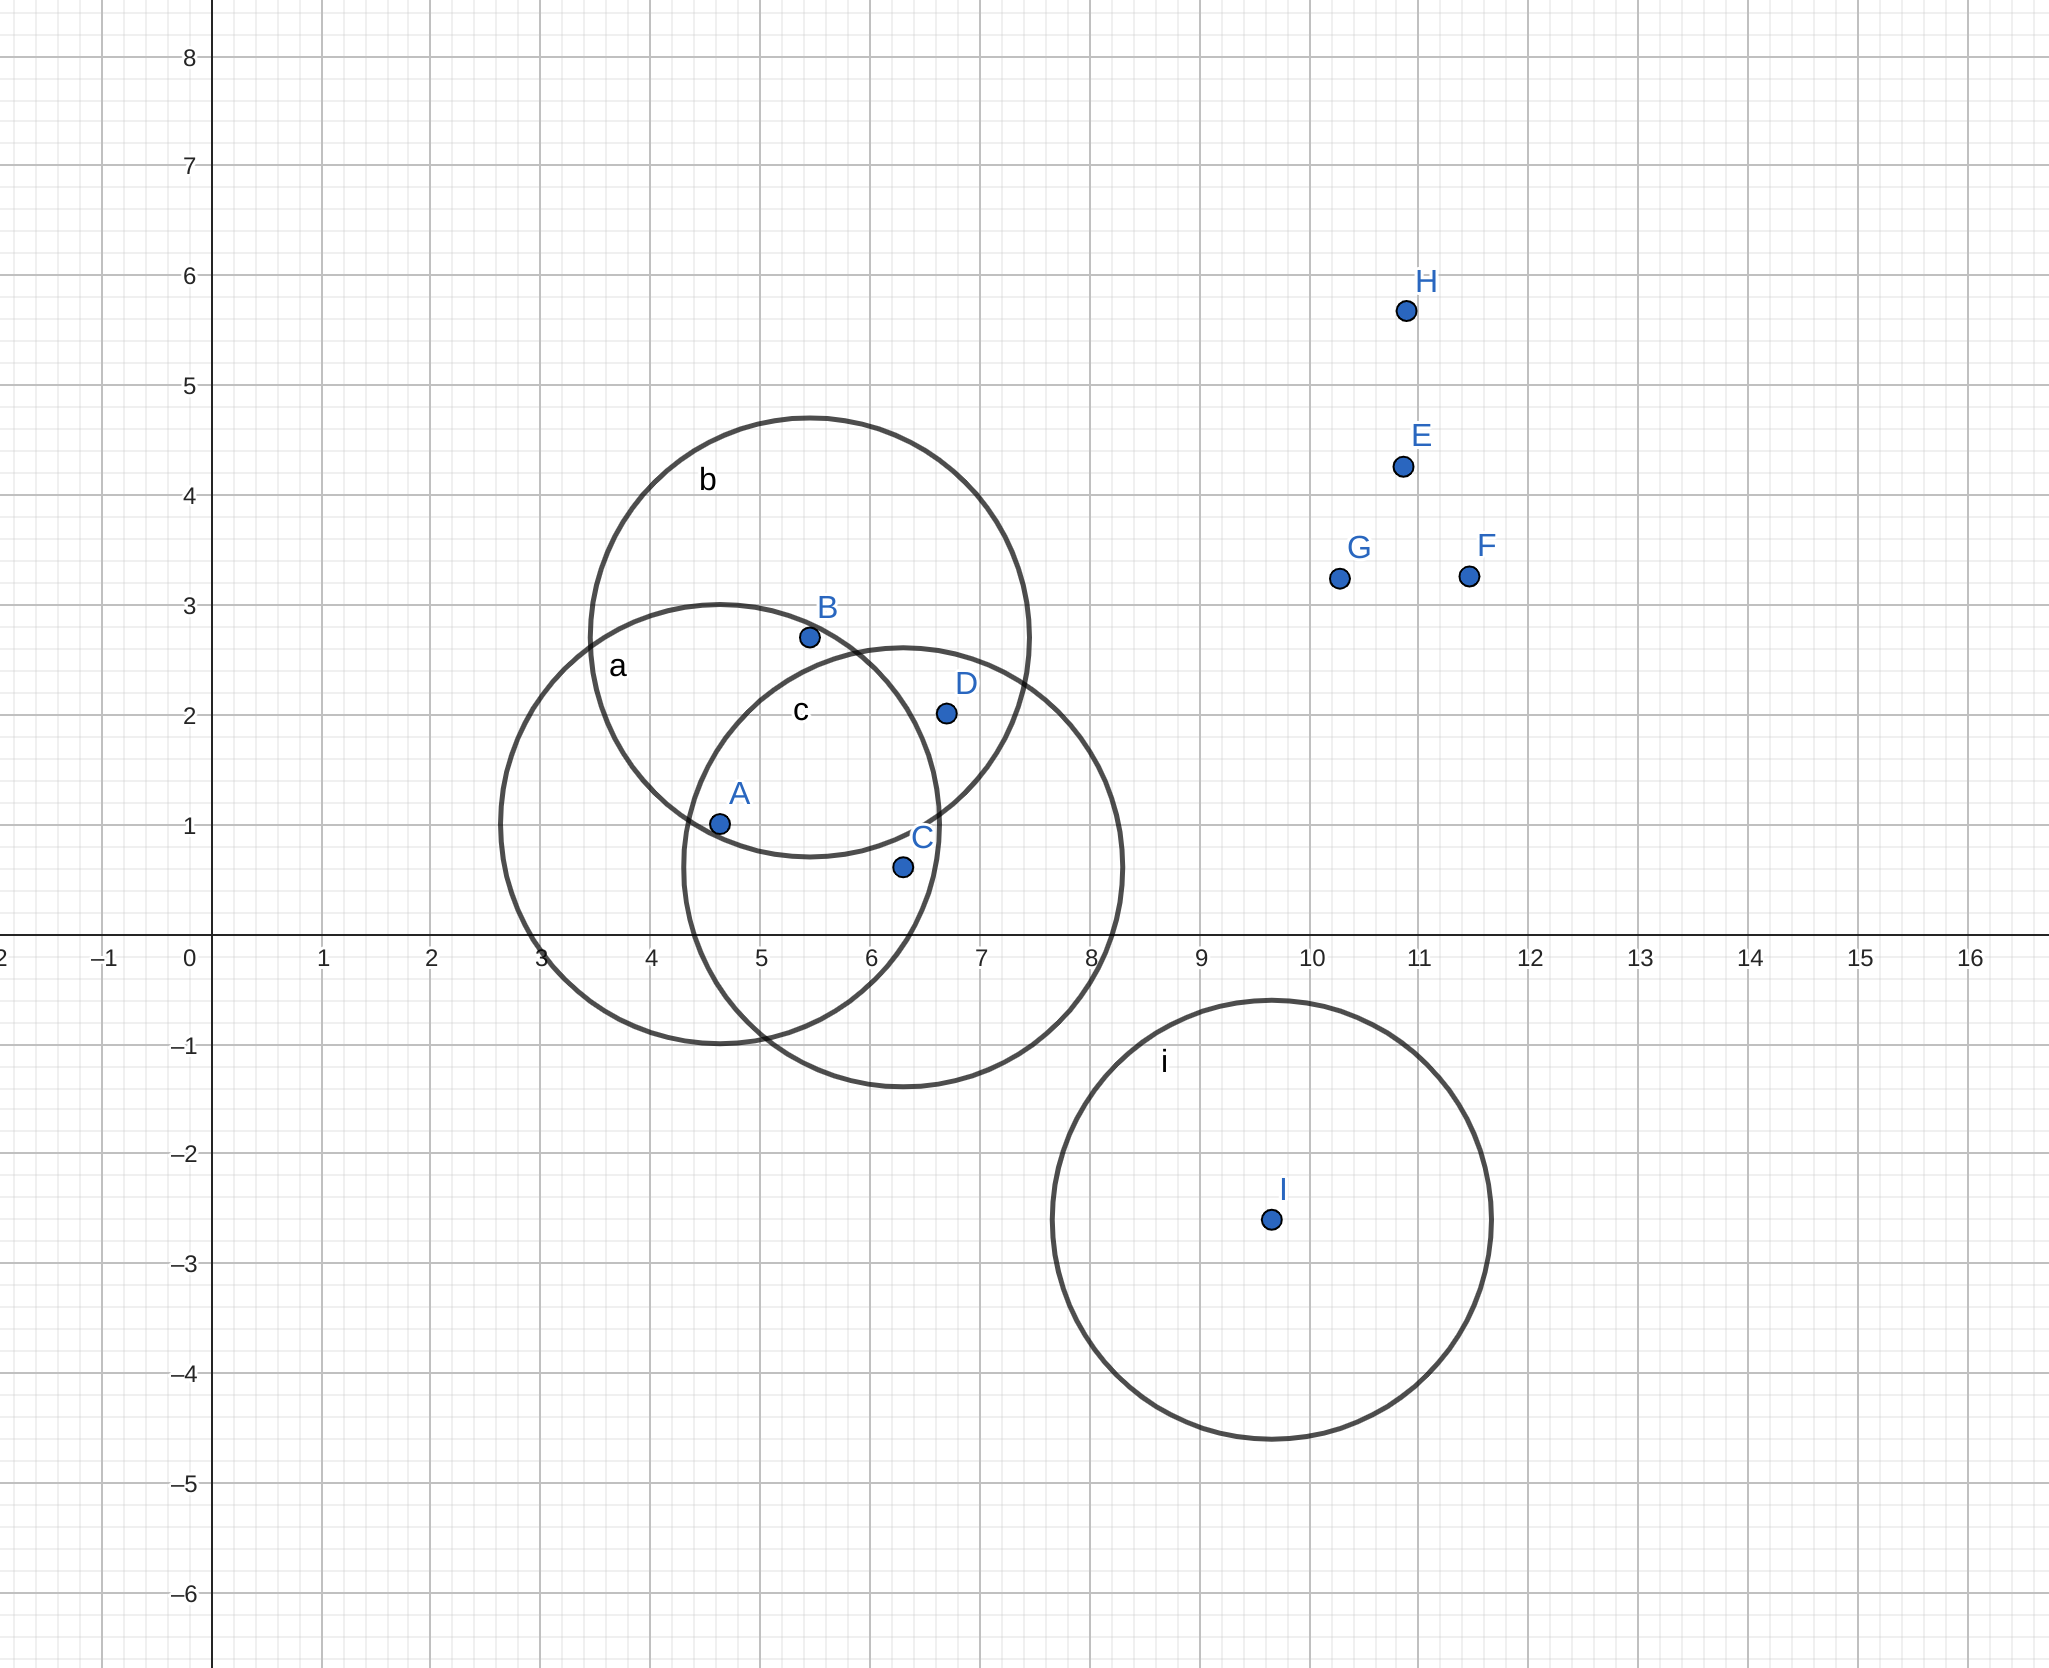
\includegraphics[height=0.41\paperheight]{images/Illustration_DBScan_1.png}
                \caption{\label{fig:ill_DBScan_1} DBScan : Détection des voisins}
            \end{figure}
        \end{column}
    \end{columns}

    \begin{table}[!ht]
        \centering
        \begin{tabular}{c|ccccc}
            \textbf{Point} & \textbf{A} & \textbf{B} & \textbf{C} & \textbf{\dots} & \textbf{I} \\ \hline
            \textbf{N(Points)} & $\left\{ A, B, C \right\}$ & $\left\{ A, B, D \right\}$ & $\left\{ A, C, D \right\}$ & & $\left\{ I \right\}$ \\ 
        \end{tabular}
    \end{table}
\end{frame}

\begin{frame}{Fonctionnement DBScan (2/2)}
    \begin{columns}
        \begin{column}{0.55\textwidth}
            \begin{block}{Etape 2 - Constuction du graphe de voisinage des noyaux}
                \begin{itemize}
                    \item Les points ayant au moins $n_{min}$ voisins sont considérés comme des noyaux. On construit alors un graphe dont les sommets sont les noyaux et il existe une arete entre deux noyaux si et seulement si ils sont voisins.
                    \item Les composantes connexes de ce graphe sont les clusters. On rattache alors aux clusters les points voisins d'au moins un noyau de ce cluster, on les appelle points de bordure.
                    \item Enfin, les sommets qui n'apparaissent pas dans le graphe sont considérés comme du bruit (pas de classe).
                \end{itemize}
            \end{block}
        \end{column}
        \begin{column}{0.45\textwidth}
            \begin{figure}
                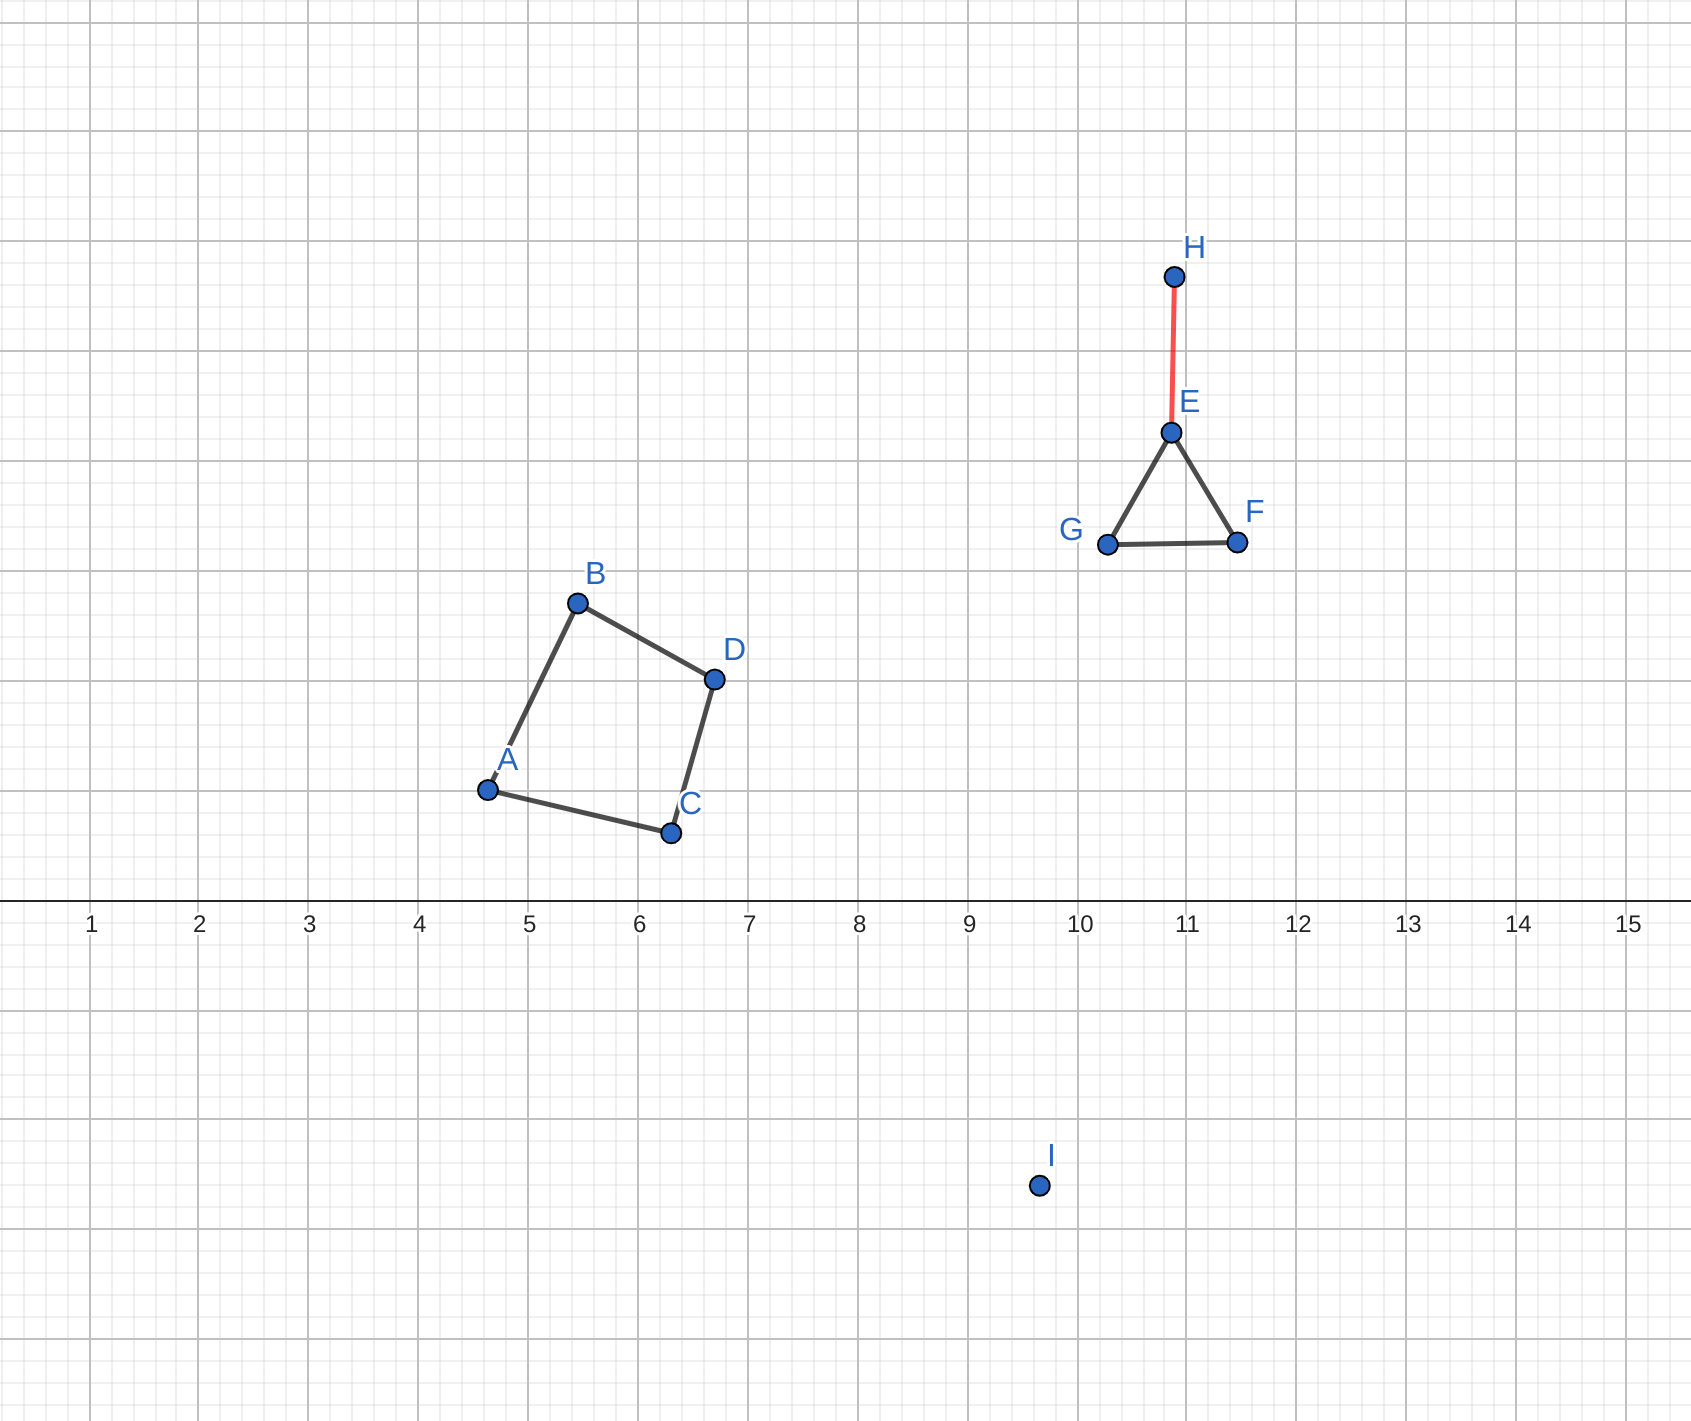
\includegraphics[height=0.5\paperheight]{images/Illustration_DBScan_2.png}
                \caption{\label{fig:ill_DBScan_2} DBScan : création des clusters}
            \end{figure}
        \end{column}
    \end{columns}
\end{frame}

\begin{frame}{Changement de métrique}
    Une façon d'améliorer le problème de mauvaise prise en compte du bruit est de changer de métrique :
    \begin{columns}
        \begin{column}{0.55\textwidth}
            \begin{block}{\emph{Core distance}}
                La \emph{core distance} d'un point du jeu de donnée est la distance entre ce point et son $k$-ième plus proche point ($k$ à fixer).
            \end{block}
        
            \begin{block}{Nouvelle métrique}
                La distance entre deux points $x$ et $y$ d'un jeu de donnée peut être définie comme la plus grande valeur entre les \emph{core distances} de $x$ et $y$ et la distance eucliedienne entre $x$ et $y$.
            \end{block}
        \end{column}
        \begin{column}{0.4\textwidth}
            \begin{figure}
                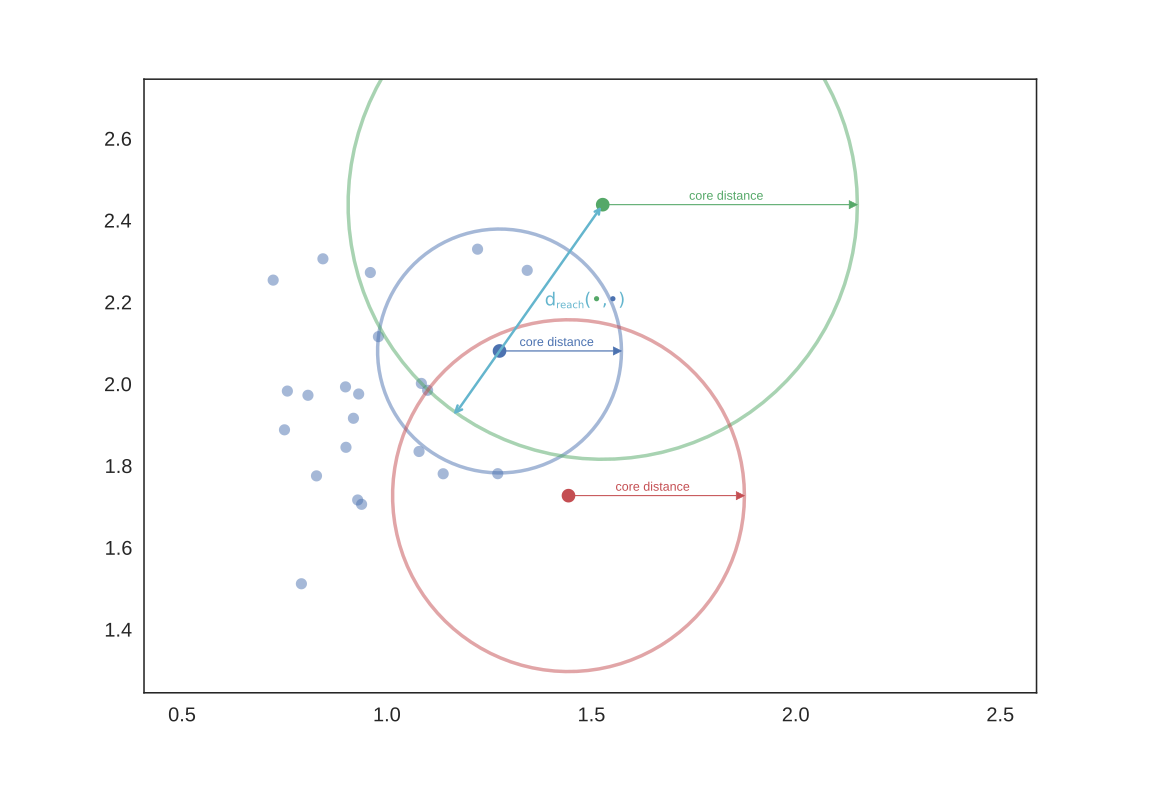
\includegraphics[width=0.6\paperheight]{images/metrique.png}
                \caption{\label{fig:metrique}Nouvelle métrique}
            \end{figure}
        \end{column}
    \end{columns}
\end{frame}



\begin{frame}{Fonctionnement HDBScan\footnotemark[2] }
    \begin{block}{Principe général}
        HDBScan consiste à fusionner les méthodes de classification hierarchique adscendante et DBScan pour permettre de s'affranchir du paramètre $\varepsilon$.
    \end{block}


    \begin{figure}
        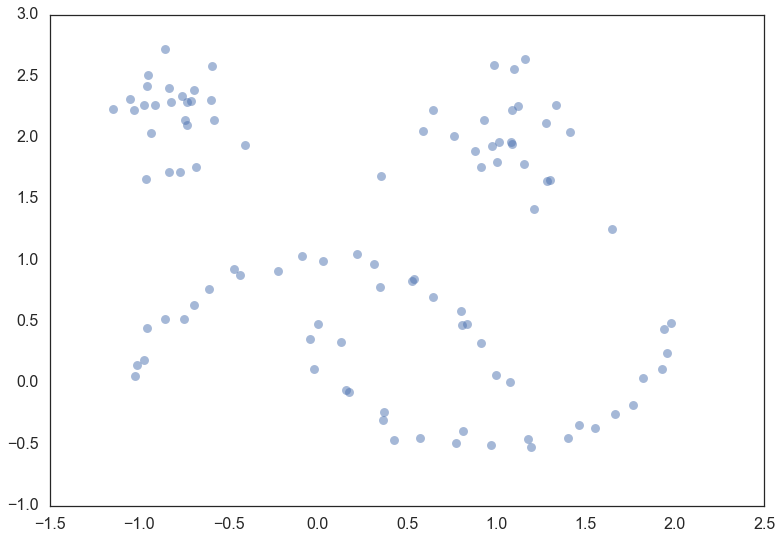
\includegraphics[width=0.5\paperheight]{images/Illustration-HDBSCAN-1.png}
        \caption{\label{fig:ill_HDBScan_1}Le jeu de donnée exemple \footnotemark[3]}
    \end{figure}

    \footnotetext[2]{\url{http://link.springer.com/chapter/10.1007\%2F978-3-642-37456-2\_14}}
    \footnotetext[3]{\url{{https://hdbscan.readthedocs.io/en/latest/how\_hdbscan_works.html}}}
\end{frame}

\begin{frame}{Fonctionnement HDBScan }
    \begin{columns}
        \begin{column}{0.55\textwidth}
            \begin{block}{Etape 1 - Constuction de l'abre couvrant de poids minimum}
                \begin{itemize}
                    \item Représenter les données par un graphe complet où chaque point est un sommet
                    \item Valuer les arêtes par la métrique expliquée précédemment;
                    \item Trouver un arbre couvrant de poids minimum dans ce graphe;
                \end{itemize}
            \end{block}
        \end{column}
        \begin{column}{0.45\textwidth}
            \begin{figure}
                \includegraphics[height=0.4\paperheight]{images/Illustration-HDBScan-2.png}
                \caption{\label{fig:ill_HDBScan_2} Arbre couvrant de poids minimum}
            \end{figure}
        \end{column}
    \end{columns}
\end{frame}

\begin{frame}{Fonctionnement HDBScan }
    \begin{columns}
        \begin{column}{0.55\textwidth}
            \begin{block}{Etape 2 - Création du dendrogramme}
                \begin{itemize}
                    \item Ne garder que les arêtes correspondant à un certain seuil que l'on fait varier.
                    \item Observer l'évolution des classes (composantes connexes) en fonction de cette distance.
                    \item Construire un dendrogramme à partir de ces informations.
                \end{itemize}
            \end{block}
        \end{column}
        \begin{column}{0.45\textwidth}
            \begin{figure}
                \includegraphics[height=0.4\paperheight]{images/Illustration-HDBScan-3.png}
                \caption{\label{fig:ill_HDBScan_3} Dendrogramme}
            \end{figure}
        \end{column}
    \end{columns}
\end{frame}

\begin{frame}{Fonctionnement HDBScan }
    \begin{columns}
        \begin{column}{0.55\textwidth}
            \begin{block}{Etape 3 - Condensation du dendrogramme}
                    On va chercher à condenser le dendrogramme précédent. Pour cela, on considère qu'au départ il n'y a qu'un cluster.
                    On considère qu'un cluster n'est plus considéré comme tel quand il possède moins d'individu qu'un certain seuil (appelons le $n_{min}$).
                    A chaque séparation dans le dendrogramme, il y'a trois cas de figure :
                    \begin{itemize}
                        \item Si les deux parties comportent au moins $n_{min}$ individus, alors on considère que le cluster parent meurt et donne naissance à deux enfants.
                        \item Si une seule des parties comporte au moins $n_{min}$ individus, alors on considère que ce cluster est la continuation du précédent.
                        \item Si les deux parties comportent moins de $n_{min}$ individus, alors on considère que le cluster meurt.
                    \end{itemize}

            \end{block}
        \end{column}
        \begin{column}{0.45\textwidth}
            \begin{figure}
                \includegraphics[height=0.4\paperheight]{images/Illustration-HDBScan-4.png}
                \caption{\label{fig:ill_HDBScan_4} Dendrogramme condensé}
            \end{figure}
        \end{column}
    \end{columns}
\end{frame}

\begin{frame}{Fonctionnement HDBScan }
    \begin{columns}
        \begin{column}{0.55\textwidth}
            \begin{block}{Etape 4 - Selection des clusters}
                    On va choisir les clusters que l'on veut grader au sein du dendrogramme condensé en choisissant les clusters les plus "durables".
                    Graphiquement, cela revient à choisir les clusters dont l'aire est la plus importante dans le dendrogramme condensé.
                    A la fin on souhaite une partition, donc qu'on ne peut selectionner à la fois un cluster et son descendant.
            \end{block}
        \end{column}
        \begin{column}{0.45\textwidth}
            \begin{figure}
                \includegraphics[height=0.4\paperheight]{images/Illustration-HDBScan-5.png}
                \caption{\label{fig:ill_HDBScan_5} Clusters choisis}
            \end{figure}
        \end{column}
    \end{columns}
\end{frame}

\begin{frame}{Fonctionnement HDBScan }
    \begin{columns}
        \begin{column}{0.55\textwidth}
            \begin{block}{Etape 5 - Resultat}
                    A la fin, on obtient les clusters ainsi qu'une probabilité pour chaque point qui caractèrise la probabilité que le point appartienne à son cluster. Cette probabilité est déterminée en observant à quel moment le point se déconnecte de son cluster dans le dengdrogramme.
            \end{block}
        \end{column}
        \begin{column}{0.45\textwidth}
            \begin{figure}
                \includegraphics[height=0.4\paperheight]{images/Illustration-HDBScan-6.png}
                \caption{\label{fig:ill_HDBScan_6} Résulats sur le jeu de donnée d'exemple}
            \end{figure}
        \end{column}
    \end{columns}
\end{frame}


\begin{frame}{HDBScan}
    \begin{block}{Avantages}
        \begin{itemize}
            \item Permet de prendre en compte les probèmes de classe à densité variable;
            \item Introduit un modèle probabiliste.
        \end{itemize}
    \end{block}

    \begin{block}{Application à notre cas d'utilisation}
        \begin{itemize}
            \item Appliqué de la même manière que DBScan : si un point est dans un cluster, alors on considère qu'il est en ville, sinon en campagne;
            \item La probabilité discutée précédemment permet de rajouter une incertitude sur l'appartenance (ou non) d'une station de base à une ville.
        \end{itemize}
    \end{block}
\end{frame}

\begin{frame}{Paramètres de sklearn.cluster.HDBSCAN \footnotemark[4]}
    \begin{itemize}
        \item \texttt{min\_cluster\_size=5} : groupings smaller than this size will be left as noise;
        \item \texttt{min\_samples=None} : The number of samples in a neighborhood for a point to be considered as a core point;
        \item \texttt{cluster\_selection\_epsilon=0.0} : Clusters below this value will be merged;
        \item \texttt{max\_cluster\_size=None};
        \item \texttt{metric='euclidean'};
        \item \texttt{metric\_params=None};
        \item \texttt{alpha=1.0} : A distance scaling parameter;
        \item \texttt{algorithm='auto'} : Exactly which algorithm to use for computing core distances;
        \item \texttt{leaf\_size=40} : Leaf size for trees responsible for fast nearest neighbour queries when a KDTree or a BallTree are used as core-distance algorithms;
        \item \texttt{n\_jobs=None} : Number of jobs to run in parallel to calculate distances;
        \item \texttt{cluster\_selection\_method='eom'} : The method used to select clusters from the condensed tree;
        \item \texttt{allow\_single\_cluster=False} : allow the result to be a single cluster;
        \item \texttt{store\_centers=None};
        \item \texttt{copy=False}.
    \end{itemize}
    \footnotetext[4]{\url{https://scikit-learn.org/stable/modules/generated/sklearn.cluster.HDBSCAN.html}}
\end{frame}

\begin{frame}{Résultats}
    \begin{figure}
        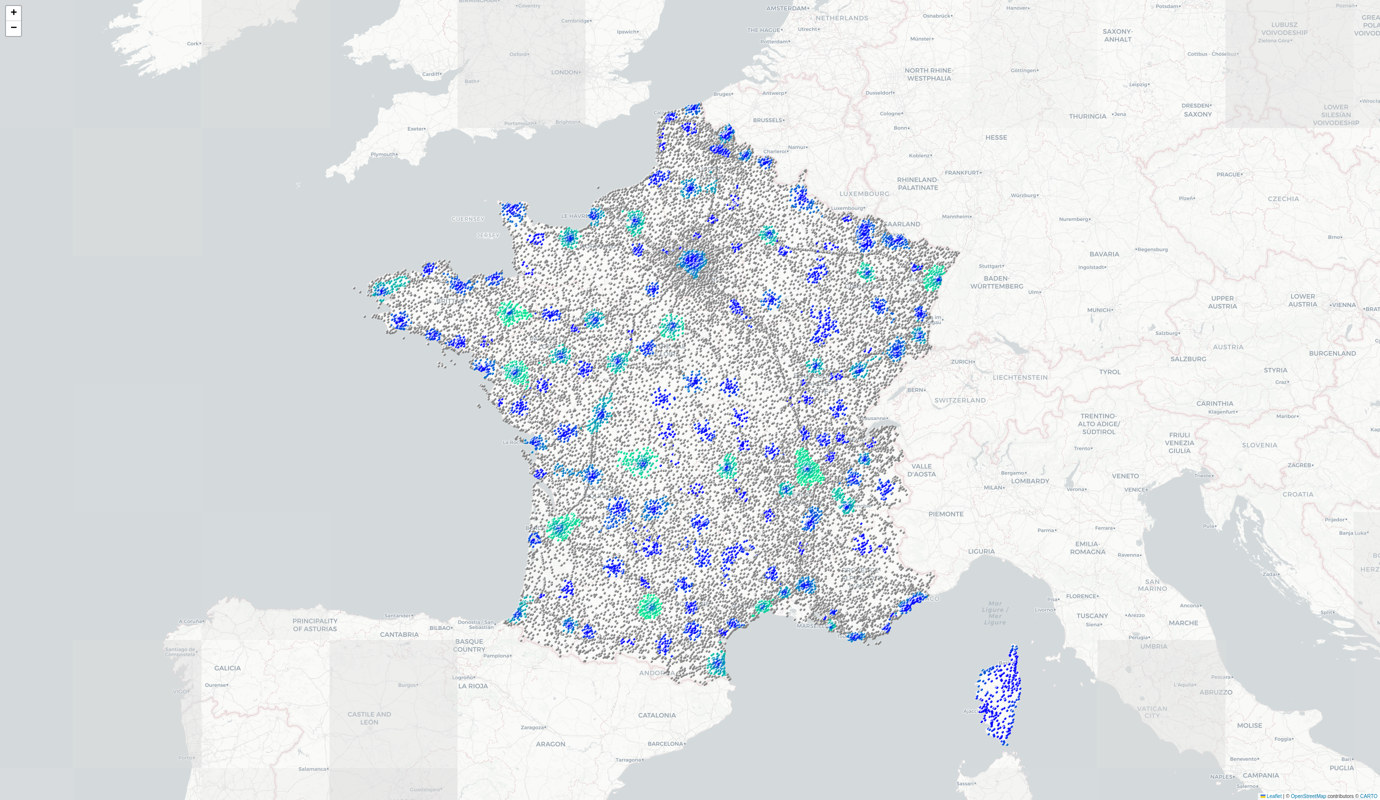
\includegraphics[width=0.9\paperheight]{images/villes_HDBSCAN.png}
        \caption{\label{fig:HDBSCAN}Application d'HDBScan \texttt{min\_cluster\_size=5}, \texttt{min\_samples=40}}
    \end{figure}
\end{frame}



